\section{Differentiable depth image warping}
\label{sec:diffwarp}

The core component of unsupervised depth learning is the differentiable depth image warp operation in the loss function of the CNN networks. Given the intrinsic camera matrix:

\[
K = 
\begin{pmatrix}
f_x & s & x_0 \\
0 & f_y & y_0 \\
0 & 0   & 1
\end{pmatrix}
\]

And the predicted depth $ D_t(p_t) $ of pixel $ p_t $ of the target (current) frame. And the transform $ T_{t \rightarrow s} $ from the target to source (next/previous) frame:

\[
T_{t \rightarrow s} =
\begin{pmatrix}
\textbf{R} & \textbf{t} \\
0 & 1
\end{pmatrix}
\]

The position of the target pixel $ p_t $ in the source image $ p_s $ can be calculated in homogeneous coordinates as:

\[
p_s \sim K T_{t \rightarrow s} D_t(p_t) K^{-1} p_t 
\]

The pixel position $ p_s $ is however continuous and in order to sample the discrete source image $ I_s $ a differentiable bilinear sampling method is used. The method is described in \textit{spatial transformer networks}\cite{spatialtransformernetworks} and works by interpolating the neighbouring 4 pixels values (top-left, bottom-right) by the distance to the the continuous sampling point $ p_t $. This process is illustrated in Figure \ref{fig:warp}.


\begin{figure}[H]
	\centering
	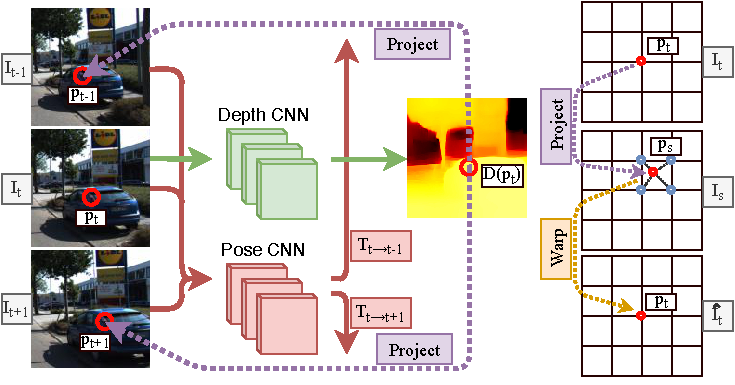
\includegraphics[width=1.0\textwidth]{warp}
	\caption{The \abbrCNN predicts the depth map $D$ of the target image $I_t$, and also the relative movement, $T_{t\rightarrow t-1}, T_{t\rightarrow t+1}$ between the target image and the source images. Each pixel $p_t$ in the target image is projected onto a position in the source images which are sampled using bilinear interpolation. This should recreate the appearance of the target image but with pixels sampled from the source image. An appearance similarity metric between the original target image and the recreated target images can be used as the loss function for the \abbrCNN to learn to accurately predict correct depth and movement.}
	\label{fig:warp}
\end{figure}

%TODO: Insert examples of warped/recreated and diff images between target and recreated images.....